
% Section: RESULTS
\section{Results}
\label{sec___results}

In this thesis, we present the complete framework of a community cloud system, 
in particular focusing on the resource allocation components.
\Cref{fig__architecture_chapters} shows how we approach this framework,
and we include the chapters and sections where we discuss different aspects of the framework.
We discuss the overall architecture
%, and the importance of resource regulation in the middleware 
in \Cref{chap__foundations}. 
We present the vision behind the community cloud system in \Cref{sec__community_clouds_background}, 
and discuss the relevance of 
the social and economic context of community networks 
in devising mechanisms to drives the adoption of the community network cloud 
in \Cref{sec__economic_mechanisms}.

At the core layer, we study how scalability affects the design of community cloud system in \Cref{sec__scalability_background}.
%
Within middleware layer, we emphasise the resource regulation components.
For a community of local users with strong social ties ensuring trust,
we propose resource regulation mechanisms in \Cref{chap__incentives}.
For larger communities which lack trust among the users, 
we propose distributed auctioneer in \Cref{chap__trusted_auction}.
Another service within middleware layer is a decision support system (DSS)
to facilitate selection of services, which we touch upon in \Cref{sec__service_selection}.
%
Within services layer, we need applications that provide utility for the members of the community network, which we discuss in \Cref{sec__cloud_services_background}.

%% FIGURE
\begin{figure}[tbp]
	\centering
	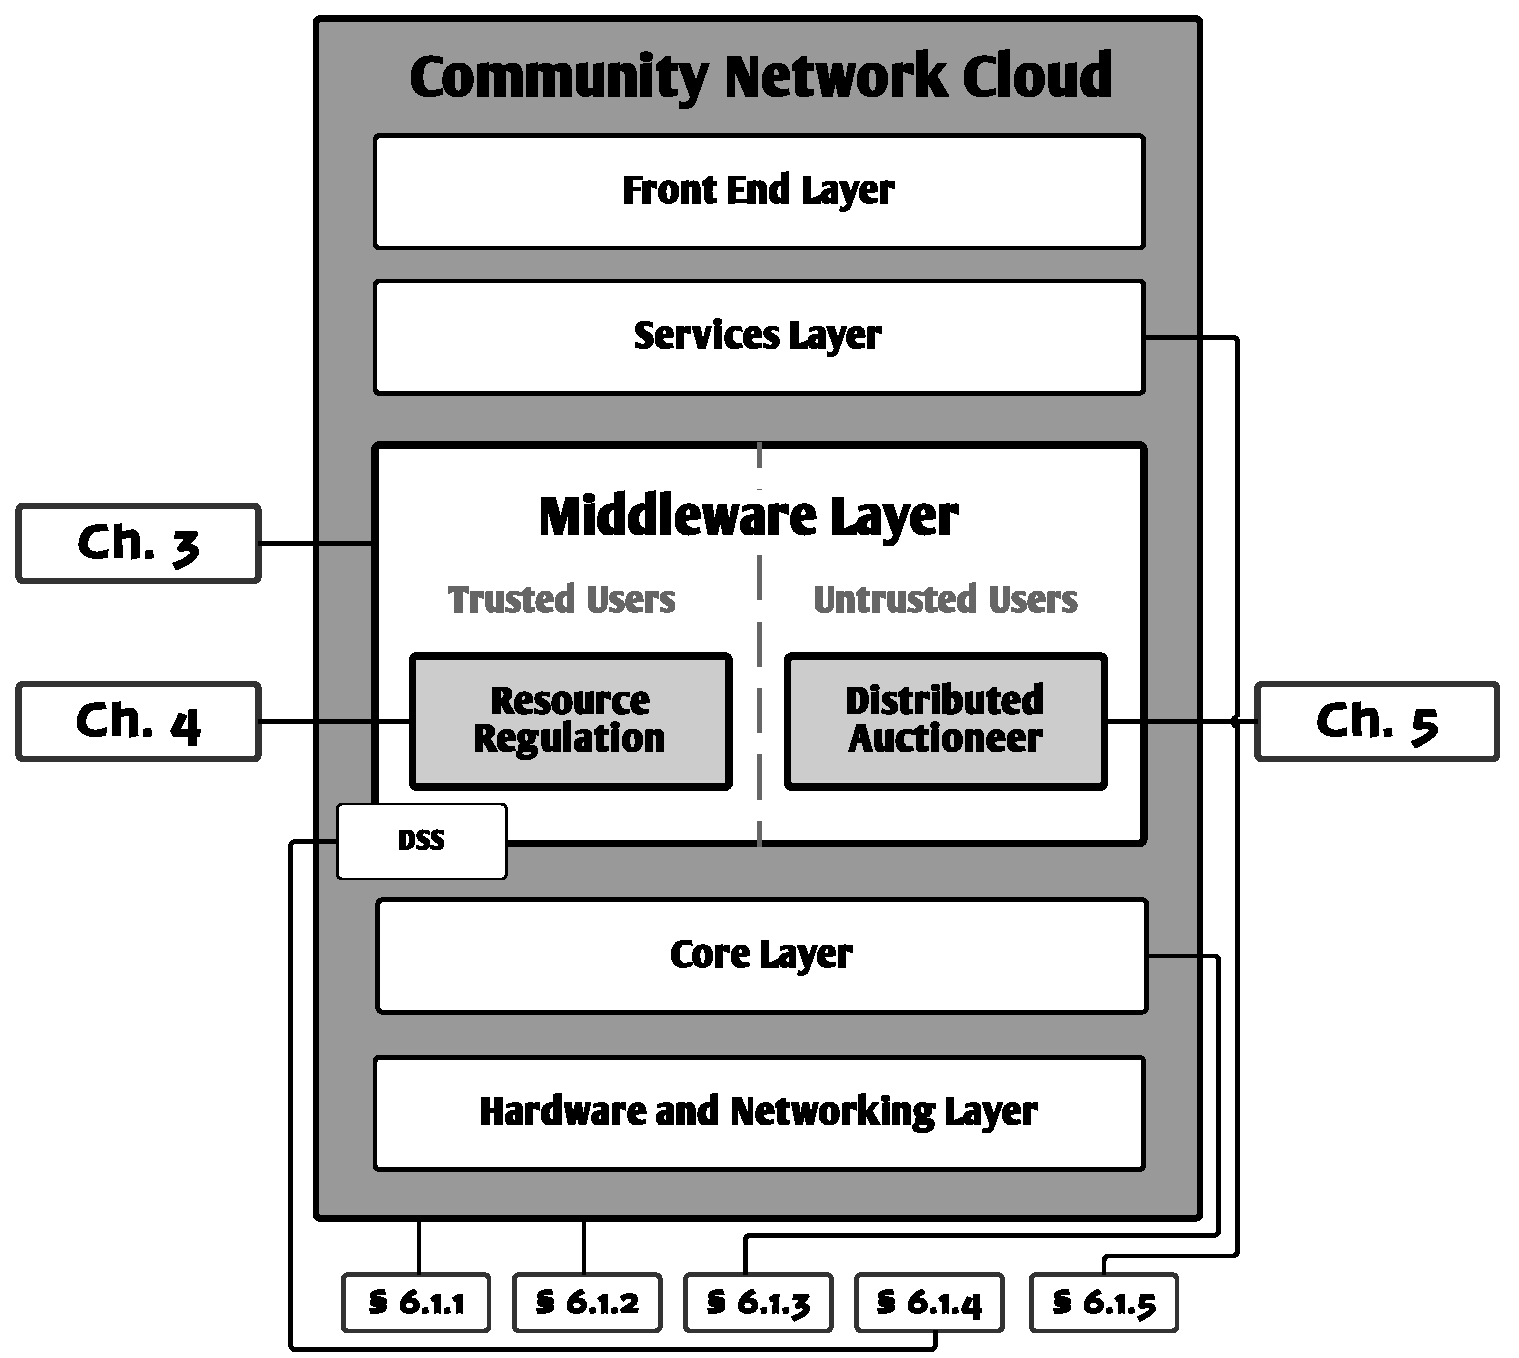
\includegraphics[width=0.8\textwidth,keepaspectratio]{architecture_chapters}
	\caption{Overview of the proposed framework}
	\label{fig__architecture_chapters}
\end{figure}

% Inspired by: http://www.gsd.inesc-id.pt/~ler/reports/filipearaujophd.pdf
% See Figure 1.1: Overview of the proposed architecture
% We can put similar figure and show relevant chapters, but also other work not in the thesis.